\documentclass[]{article}
\usepackage{lmodern}
\usepackage{amssymb,amsmath}
\usepackage{ifxetex,ifluatex}
\usepackage{fixltx2e} % provides \textsubscript
\ifnum 0\ifxetex 1\fi\ifluatex 1\fi=0 % if pdftex
  \usepackage[T1]{fontenc}
  \usepackage[utf8]{inputenc}
\else % if luatex or xelatex
  \ifxetex
    \usepackage{mathspec}
  \else
    \usepackage{fontspec}
  \fi
  \defaultfontfeatures{Ligatures=TeX,Scale=MatchLowercase}
\fi
% use upquote if available, for straight quotes in verbatim environments
\IfFileExists{upquote.sty}{\usepackage{upquote}}{}
% use microtype if available
\IfFileExists{microtype.sty}{%
\usepackage{microtype}
\UseMicrotypeSet[protrusion]{basicmath} % disable protrusion for tt fonts
}{}
\usepackage[margin=1in]{geometry}
\usepackage{hyperref}
\hypersetup{unicode=true,
            pdftitle={Curs Biostatistica 2017 - Laborator 9 \& 10},
            pdfborder={0 0 0},
            breaklinks=true}
\urlstyle{same}  % don't use monospace font for urls
\usepackage{color}
\usepackage{fancyvrb}
\newcommand{\VerbBar}{|}
\newcommand{\VERB}{\Verb[commandchars=\\\{\}]}
\DefineVerbatimEnvironment{Highlighting}{Verbatim}{commandchars=\\\{\}}
% Add ',fontsize=\small' for more characters per line
\usepackage{framed}
\definecolor{shadecolor}{RGB}{248,248,248}
\newenvironment{Shaded}{\begin{snugshade}}{\end{snugshade}}
\newcommand{\KeywordTok}[1]{\textcolor[rgb]{0.13,0.29,0.53}{\textbf{{#1}}}}
\newcommand{\DataTypeTok}[1]{\textcolor[rgb]{0.13,0.29,0.53}{{#1}}}
\newcommand{\DecValTok}[1]{\textcolor[rgb]{0.00,0.00,0.81}{{#1}}}
\newcommand{\BaseNTok}[1]{\textcolor[rgb]{0.00,0.00,0.81}{{#1}}}
\newcommand{\FloatTok}[1]{\textcolor[rgb]{0.00,0.00,0.81}{{#1}}}
\newcommand{\ConstantTok}[1]{\textcolor[rgb]{0.00,0.00,0.00}{{#1}}}
\newcommand{\CharTok}[1]{\textcolor[rgb]{0.31,0.60,0.02}{{#1}}}
\newcommand{\SpecialCharTok}[1]{\textcolor[rgb]{0.00,0.00,0.00}{{#1}}}
\newcommand{\StringTok}[1]{\textcolor[rgb]{0.31,0.60,0.02}{{#1}}}
\newcommand{\VerbatimStringTok}[1]{\textcolor[rgb]{0.31,0.60,0.02}{{#1}}}
\newcommand{\SpecialStringTok}[1]{\textcolor[rgb]{0.31,0.60,0.02}{{#1}}}
\newcommand{\ImportTok}[1]{{#1}}
\newcommand{\CommentTok}[1]{\textcolor[rgb]{0.56,0.35,0.01}{\textit{{#1}}}}
\newcommand{\DocumentationTok}[1]{\textcolor[rgb]{0.56,0.35,0.01}{\textbf{\textit{{#1}}}}}
\newcommand{\AnnotationTok}[1]{\textcolor[rgb]{0.56,0.35,0.01}{\textbf{\textit{{#1}}}}}
\newcommand{\CommentVarTok}[1]{\textcolor[rgb]{0.56,0.35,0.01}{\textbf{\textit{{#1}}}}}
\newcommand{\OtherTok}[1]{\textcolor[rgb]{0.56,0.35,0.01}{{#1}}}
\newcommand{\FunctionTok}[1]{\textcolor[rgb]{0.00,0.00,0.00}{{#1}}}
\newcommand{\VariableTok}[1]{\textcolor[rgb]{0.00,0.00,0.00}{{#1}}}
\newcommand{\ControlFlowTok}[1]{\textcolor[rgb]{0.13,0.29,0.53}{\textbf{{#1}}}}
\newcommand{\OperatorTok}[1]{\textcolor[rgb]{0.81,0.36,0.00}{\textbf{{#1}}}}
\newcommand{\BuiltInTok}[1]{{#1}}
\newcommand{\ExtensionTok}[1]{{#1}}
\newcommand{\PreprocessorTok}[1]{\textcolor[rgb]{0.56,0.35,0.01}{\textit{{#1}}}}
\newcommand{\AttributeTok}[1]{\textcolor[rgb]{0.77,0.63,0.00}{{#1}}}
\newcommand{\RegionMarkerTok}[1]{{#1}}
\newcommand{\InformationTok}[1]{\textcolor[rgb]{0.56,0.35,0.01}{\textbf{\textit{{#1}}}}}
\newcommand{\WarningTok}[1]{\textcolor[rgb]{0.56,0.35,0.01}{\textbf{\textit{{#1}}}}}
\newcommand{\AlertTok}[1]{\textcolor[rgb]{0.94,0.16,0.16}{{#1}}}
\newcommand{\ErrorTok}[1]{\textcolor[rgb]{0.64,0.00,0.00}{\textbf{{#1}}}}
\newcommand{\NormalTok}[1]{{#1}}
\usepackage{longtable,booktabs}
\usepackage{graphicx,grffile}
\makeatletter
\def\maxwidth{\ifdim\Gin@nat@width>\linewidth\linewidth\else\Gin@nat@width\fi}
\def\maxheight{\ifdim\Gin@nat@height>\textheight\textheight\else\Gin@nat@height\fi}
\makeatother
% Scale images if necessary, so that they will not overflow the page
% margins by default, and it is still possible to overwrite the defaults
% using explicit options in \includegraphics[width, height, ...]{}
\setkeys{Gin}{width=\maxwidth,height=\maxheight,keepaspectratio}
\IfFileExists{parskip.sty}{%
\usepackage{parskip}
}{% else
\setlength{\parindent}{0pt}
\setlength{\parskip}{6pt plus 2pt minus 1pt}
}
\setlength{\emergencystretch}{3em}  % prevent overfull lines
\providecommand{\tightlist}{%
  \setlength{\itemsep}{0pt}\setlength{\parskip}{0pt}}
\setcounter{secnumdepth}{5}
% Redefines (sub)paragraphs to behave more like sections
\ifx\paragraph\undefined\else
\let\oldparagraph\paragraph
\renewcommand{\paragraph}[1]{\oldparagraph{#1}\mbox{}}
\fi
\ifx\subparagraph\undefined\else
\let\oldsubparagraph\subparagraph
\renewcommand{\subparagraph}[1]{\oldsubparagraph{#1}\mbox{}}
\fi

%%% Use protect on footnotes to avoid problems with footnotes in titles
\let\rmarkdownfootnote\footnote%
\def\footnote{\protect\rmarkdownfootnote}

%%% Change title format to be more compact
\usepackage{titling}

% Create subtitle command for use in maketitle
\newcommand{\subtitle}[1]{
  \posttitle{
    \begin{center}\large#1\end{center}
    }
}

\setlength{\droptitle}{-2em}
  \title{Curs Biostatistica 2017 - Laborator 9 \& 10}
  \pretitle{\vspace{\droptitle}\centering\huge}
  \posttitle{\par}
\subtitle{Regresie}
  \author{}
  \preauthor{}\postauthor{}
  \date{}
  \predate{}\postdate{}

\usepackage{booktabs}
\usepackage{longtable}
\usepackage{framed,color}
\definecolor{shadecolor}{RGB}{248,248,248}

\ifxetex
  \usepackage{letltxmacro}
  \setlength{\XeTeXLinkMargin}{1pt}
  \LetLtxMacro\SavedIncludeGraphics\includegraphics
  \def\includegraphics#1#{% #1 catches optional stuff (star/opt. arg.)
    \IncludeGraphicsAux{#1}%
  }%
  \newcommand*{\IncludeGraphicsAux}[2]{%
    \XeTeXLinkBox{%
      \SavedIncludeGraphics#1{#2}%
    }%
  }%
\fi

\newenvironment{rmdblock}[1]
  {\begin{shaded*}
  \begin{itemize}
  \renewcommand{\labelitemi}{
    \raisebox{-.7\height}[0pt][0pt]{
      {\setkeys{Gin}{width=2em,keepaspectratio}\includegraphics{images/icons/#1}}
    }
  }
  \item
  }
  {
  \end{itemize}
  \end{shaded*}
  }
\newenvironment{rmdcaution}
  {\begin{rmdblock}{caution}}
  {\end{rmdblock}}
\newenvironment{rmdinsight}
  {\begin{rmdblock}{insight}}
  {\end{rmdblock}}
\newenvironment{rmdexercise}
  {\begin{rmdblock}{exercise}}
  {\end{rmdblock}}
\newenvironment{rmdtip}
  {\begin{rmdblock}{tip}}
  {\end{rmdblock}}

\begin{document}
\maketitle

{
\setcounter{tocdepth}{2}
\tableofcontents
}
\section{Regresie liniară multiplă}\label{regresie-liniara-multipla}

\begin{center}\rule{0.5\linewidth}{\linethickness}\end{center}

\begin{center}\rule{0.5\linewidth}{\linethickness}\end{center}

\subsection{Introducere}\label{introducere}

Modelul de regresie liniară multiplă reprezintă o generalizare a
modelului de regresie simplă. Dacă în regresia liniară simplă se folosea
o singură variabilă predictor \(X\) ca să explice variabila răspuns
\(Y\), în modelul de regresie liniară multiplă se folosesc mai multe
variabile predictor \(X_1,\ldots,X_k\) pentru a explica răspunsul \(Y\):

\[
\mathbb{E}[Y|X_1 = x_1, \ldots, X_k=x_x]=\beta_0+\beta_1x_1+\beta_2x_2+\ldots+\beta_kx_k
\] sau altfel scris

\[
Y = \beta_0 + \beta_1 X_1 + \ldots + \beta_k X_k + \varepsilon.
\]

Date fiind observațiile actuale, cu alte cuvinte dat fiind un eșantion
\((X_{11},\ldots,X_{1k},Y_1),\ldots,(X_{n1},\ldots,X_{nk},Y_n)\) al lui
\((X_1,\ldots,X_k,Y)\), unde \(X_{ij}\) reprezintă a \(i\)-a observație
a predictorului \(X_j\), modelul se poate scrie

\[
y_i = \beta_0+\beta_1x_{i1}+\beta_2x_{i2}+\ldots+\beta_kx_{ik}+\varepsilon_i, \quad i = 1,\ldots,n
\]

a cărui formă compactă (matriceală) este

\[
\mathbf{Y}=\mathbf{X}\boldsymbol\beta+\boldsymbol\varepsilon
\]

\begin{itemize}
\tightlist
\item
  \(\mathbf{X}\) este \emph{matricea de design}
\end{itemize}

\[
\mathbf{X}=\begin{pmatrix}
1 & X_{11} & \cdots & X_{1k}\\
\vdots & \vdots & \ddots & \vdots\\
1 & X_{n1} & \cdots & X_{nk}
\end{pmatrix}_{n\times(k+1)}
\]

\begin{itemize}
\tightlist
\item
  \(\mathbf{Y}\) este \emph{vectorul răspuns}, \(\boldsymbol\beta\) este
  \emph{vectorul coeficienților} iar \(\boldsymbol\varepsilon\) este
  \emph{vectorul eroare}
\end{itemize}

\[
\mathbf{Y}=\begin{pmatrix}
Y_1 \\
\vdots \\
Y_n
\end{pmatrix}_{n\times 1},\quad\boldsymbol\beta=\begin{pmatrix}
\beta_0 \\
\beta_1 \\
\vdots \\
\beta_k
\end{pmatrix}_{(k+1)\times 1}\text{ și }\quad
\boldsymbol\varepsilon=\begin{pmatrix}
\varepsilon_1 \\
\vdots \\
\varepsilon_n
\end{pmatrix}_{n\times 1}.
\]

\begin{rmdinsight}
Să observăm că pentru \(k=1\) modelul se reduce la regresia liniară
simplă. În acest caz:

\[
\mathbf{X}=\begin{pmatrix}
1 & X_{11}\\
\vdots & \vdots\\
1 & X_{n1}
\end{pmatrix}_{n\times2}\text{ și }\quad \beta=\begin{pmatrix}
\beta_0 \\
\beta_1 
\end{pmatrix}_{2\times 1}
\]
\end{rmdinsight}

\emph{Suma abaterilor pătratice reziduale} pentru modelul de regresie
liniară multiplă este

\[
RSS(\boldsymbol\beta)=\sum_{i=1}^n(Y_i-\beta_0-\beta_1X_{i1}-\ldots-\beta_kX_{ik})^2=(\mathbf{Y}-\mathbf{X}\boldsymbol{\beta})^T(\mathbf{Y}-\mathbf{X}\boldsymbol{\beta})
\]

ceea ce conduce la \emph{sistemul de ecuații normale}

\[
\mathbf{X}^\intercal\mathbf{X}\hat{\boldsymbol{\beta}}=\mathbf{X}^\intercal\mathbf{Y}
\]

a cărui soluție, dat fiind că \(\mathbf{X}^\intercal\mathbf{X}\) este
inversabilă, este

\[
\hat{\boldsymbol{\beta}}=(\mathbf{X}^\intercal\mathbf{X})^{-1}\mathbf{X}^\intercal\mathbf{Y}
\]

Odată ce avem estimatorul \(\hat{\boldsymbol{\beta}}\) , putem defini:

\begin{itemize}
\tightlist
\item
  \emph{valorile prognozate} (\emph{fitted values})
  \(\hat Y_1,\ldots,\hat Y_n\) (valorile verticale pe hiperplanul de
  regresie), unde
\end{itemize}

\[
\hat Y_i=\hat\beta_0+\hat\beta_1X_{i1}+\cdots+\hat\beta_kX_{ik},\quad i=1,\ldots,n
\]

și sub formă matriceală

\[
\hat{\mathbf{Y}}=\mathbf{X}\hat{\boldsymbol{\beta}}=\mathbf{X}(\mathbf{X}^\intercal\mathbf{X})^{-1}\mathbf{X}^\intercal\mathbf{Y}=\mathbf{H}\mathbf{Y}
\]

unde
\(\mathbf{H}=\mathbf{X}(\mathbf{X}^\intercal\mathbf{X})^{-1}\mathbf{X}^\intercal\)
se numește \emph{matricea căciulă} (\emph{hat matrix}) și reprezintă
proiecția ortogonală a lui \(\mathbf{Y}\) în spațiul generat de
\(\mathbf{X}\).

\begin{itemize}
\tightlist
\item
  \emph{reziduurile estimate} (\emph{estimated residuals})
  \(\hat \varepsilon_1,\ldots,\hat \varepsilon_n\), unde
\end{itemize}

\[
\hat\varepsilon_i=Y_i-\hat Y_i,\quad i=1,\ldots,n
\]

și sub formă matriceală

\[
\hat{\boldsymbol\varepsilon} = \boldsymbol Y - \hat{\boldsymbol Y} = (\boldsymbol I-\boldsymbol H)\boldsymbol Y
\]

\begin{figure}

{\centering 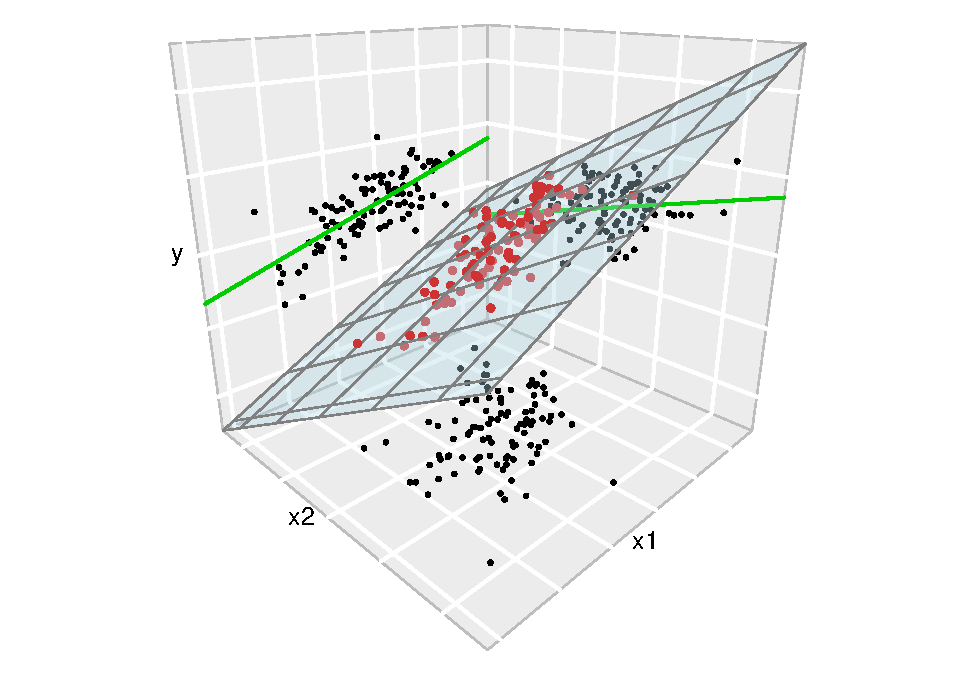
\includegraphics[width=0.9\linewidth]{Lab_9_10_files/figure-latex/unnamed-chunk-3-1} 

}

\caption{Planul de regresie (albastru) si relatia cu regresiile liniare simple (liniile verzi). Punctele rosii reprezinta un esantion pentru $(X_1,X_2,Y)$ iar punctele negre sunt subesantioane pentru $(X_1,X_2)$ (la baza), $(X_1,Y)$ (stanga) si $(X_2,Y)$ (dreapta).}\label{fig:unnamed-chunk-3}
\end{figure}

Ipotezele modelului sunt:

\begin{enumerate}
\def\labelenumi{\roman{enumi}.}
\tightlist
\item
  \textbf{Linearitatea}:
  \(\mathbb{E}[Y|X_1=x_1,\ldots,X_k=x_k]=\beta_0+\beta_1x_1+\ldots+\beta_kx_k\)
\item
  \textbf{Homoscedasticitatea}:
  \(\mathbb{V}\text{ar}(\varepsilon_i)=\sigma^2\), cu \(\sigma^2\)
  constantă pentru \(i=1,\ldots,n\)
\item
  \textbf{Normalitatea}: \(\varepsilon_i\sim\mathcal{N}(0,\sigma^2)\)
  pentru \(i=1,\ldots,n\)
\item
  \textbf{Independența erorilor}: \(\varepsilon_1,\ldots,\varepsilon_n\)
  sunt independente (sau necorelate,
  \(\mathbb{E}[\varepsilon_i\varepsilon_j]=0\), \(i\neq j\), deoarece
  sunt presupuse normale)
\end{enumerate}

Altfel spus

\[
Y|(X_1=x_1,\ldots,X_k=x_k)\sim \mathcal{N}(\beta_0+\beta_1x_1+\ldots+\beta_kx_k,\sigma^2)
\]

\textbackslash{}begin\{figure\}

\{\centering 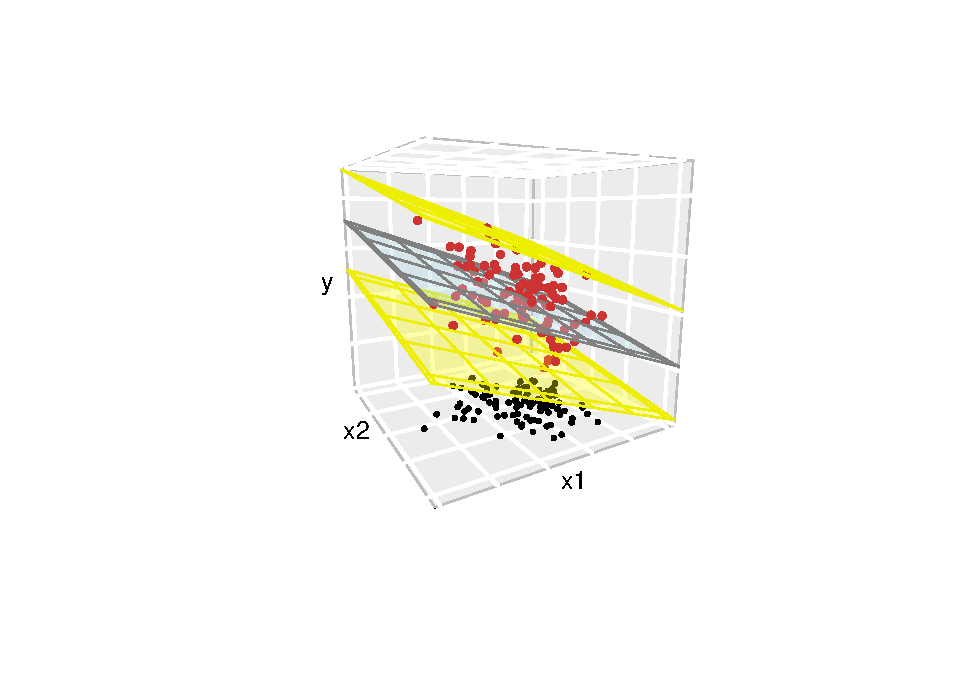
\includegraphics[width=0.9\linewidth]{Lab_9_10_files/figure-latex/unnamed-chunk-4-1}

\}

\textbackslash{}caption\{Planul de regresie. Spatiul dintre cele doua
plane galbene arata unde se afla 95\% din observatii (dupa modelul
ales).\}\label{fig:unnamed-chunk-4} \textbackslash{}end\{figure\}

Estimatorul pentru \(\sigma^2\) este

\[
\hat{\sigma}^2 = \frac{RSS(\hat{\beta}_0,\hat{\beta}_1,\ldots, \hat{\beta}_k))}{n-(k+1)} = \frac{\hat{\boldsymbol \varepsilon}^\intercal\hat{\boldsymbol \varepsilon}}{n-(k+1)} = \frac{\sum_{i=1}^{n}\hat{\varepsilon}_i^2}{n-(k+1)}.
\]

\subsection{Exemplul 1}\label{exemplul-1}

\begin{quote}
Considerăm setul de date \href{data/galapagos.csv}{\texttt{galapagos}}
care conține informații despre numărul de specii de broaște țestoase din
diferite insule din arhipelagul Galapagos (vezi
\href{http://science.sciencemag.org/content/179/4076/893.long}{articol}).
Setul conține date din 30 de insule despre numărul de specii de țestoase
(\texttt{Species}), numărul de specii endemice (\texttt{Endemics}),
suprafața insulei (\texttt{Area}), înălțimea maximă a insulei
(`\texttt{Elevation}), distanța la cea mai apropiată insulă
(\texttt{Nearest}), distanța față de insula Snata Cruz (\texttt{Scruz})
și suprafața insulei adiacente (\texttt{Adjacent}). Vrem să investigăm
relația liniară dintre numărul de specii și celelalte variabile.
\end{quote}

Începem prin a citi datele

\begin{Shaded}
\begin{Highlighting}[]
\CommentTok{# gala = read.csv("data/galapagos.csv")}

\KeywordTok{data}\NormalTok{(}\StringTok{"gala"}\NormalTok{) }\CommentTok{# este nevoie de libraria faraway}
\KeywordTok{head}\NormalTok{(gala)}
\end{Highlighting}
\end{Shaded}

\begin{verbatim}
##              Species Endemics  Area Elevation Nearest Scruz Adjacent
## Baltra            58       23 25.09       346     0.6   0.6     1.84
## Bartolome         31       21  1.24       109     0.6  26.3   572.33
## Caldwell           3        3  0.21       114     2.8  58.7     0.78
## Champion          25        9  0.10        46     1.9  47.4     0.18
## Coamano            2        1  0.05        77     1.9   1.9   903.82
## Daphne.Major      18       11  0.34       119     8.0   8.0     1.84
\end{verbatim}

Considerăm modelul de regresie liniară multiplă cu 5 predictori:

\begin{Shaded}
\begin{Highlighting}[]
\NormalTok{gala_model =}\StringTok{ }\KeywordTok{lm}\NormalTok{(Species ~}\StringTok{ }\NormalTok{Area +}\StringTok{ }\NormalTok{Elevation +}\StringTok{ }\NormalTok{Nearest +}\StringTok{ }\NormalTok{Scruz +}\StringTok{ }\NormalTok{Adjacent, }\DataTypeTok{data=}\NormalTok{gala)}

\NormalTok{gala_model_summary =}\StringTok{ }\KeywordTok{summary}\NormalTok{(gala_model)}
\NormalTok{gala_model_summary}
\end{Highlighting}
\end{Shaded}

\begin{verbatim}
## 
## Call:
## lm(formula = Species ~ Area + Elevation + Nearest + Scruz + Adjacent, 
##     data = gala)
## 
## Residuals:
##      Min       1Q   Median       3Q      Max 
## -111.679  -34.898   -7.862   33.460  182.584 
## 
## Coefficients:
##              Estimate Std. Error t value Pr(>|t|)    
## (Intercept)  7.068221  19.154198   0.369 0.715351    
## Area        -0.023938   0.022422  -1.068 0.296318    
## Elevation    0.319465   0.053663   5.953 3.82e-06 ***
## Nearest      0.009144   1.054136   0.009 0.993151    
## Scruz       -0.240524   0.215402  -1.117 0.275208    
## Adjacent    -0.074805   0.017700  -4.226 0.000297 ***
## ---
## Signif. codes:  0 '***' 0.001 '**' 0.01 '*' 0.05 '.' 0.1 ' ' 1
## 
## Residual standard error: 60.98 on 24 degrees of freedom
## Multiple R-squared:  0.7658, Adjusted R-squared:  0.7171 
## F-statistic:  15.7 on 5 and 24 DF,  p-value: 6.838e-07
\end{verbatim}

\subsubsection{Estimarea parametrilor}\label{estimarea-parametrilor}

Pentru început extragem matricea de design \(X\)

\begin{Shaded}
\begin{Highlighting}[]
\NormalTok{X =}\StringTok{ }\KeywordTok{model.matrix}\NormalTok{( ~}\StringTok{ }\NormalTok{Area +}\StringTok{ }\NormalTok{Elevation +}\StringTok{ }\NormalTok{Nearest +}\StringTok{ }\NormalTok{Scruz +}\StringTok{ }\NormalTok{Adjacent, }
    \DataTypeTok{data =} \NormalTok{gala)}

\KeywordTok{head}\NormalTok{(X)}
\end{Highlighting}
\end{Shaded}

\begin{verbatim}
##              (Intercept)  Area Elevation Nearest Scruz Adjacent
## Baltra                 1 25.09       346     0.6   0.6     1.84
## Bartolome              1  1.24       109     0.6  26.3   572.33
## Caldwell               1  0.21       114     2.8  58.7     0.78
## Champion               1  0.10        46     1.9  47.4     0.18
## Coamano                1  0.05        77     1.9   1.9   903.82
## Daphne.Major           1  0.34       119     8.0   8.0     1.84
\end{verbatim}

și răspunsul \(y\)

\begin{Shaded}
\begin{Highlighting}[]
\NormalTok{y =}\StringTok{ }\NormalTok{gala$Species}
\end{Highlighting}
\end{Shaded}

Vrem să găsim
\(\hat{\boldsymbol{\beta}}=(\mathbf{X}^\intercal\mathbf{X})^{-1}\mathbf{X}^\intercal\mathbf{Y}\)

\begin{Shaded}
\begin{Highlighting}[]
\CommentTok{# determinam (\textbackslash{}mathbf\{X\}^\textbackslash{}intercal\textbackslash{}mathbf\{X\})^\{-1\}}

\NormalTok{xtxi =}\StringTok{ }\KeywordTok{solve}\NormalTok{(}\KeywordTok{t}\NormalTok{(X) %*%}\StringTok{ }\NormalTok{X) }\CommentTok{# t() - este transpusa}
                         \CommentTok{# %*% - produsul matriceal}
                         \CommentTok{# solve() - calculeaza pseudoinversa}

\NormalTok{bHat =}\StringTok{ }\NormalTok{xtxi %*%}\StringTok{ }\KeywordTok{t}\NormalTok{(X) %*%}\StringTok{ }\NormalTok{y}
\NormalTok{bHat}
\end{Highlighting}
\end{Shaded}

\begin{verbatim}
##                     [,1]
## (Intercept)  7.068220709
## Area        -0.023938338
## Elevation    0.319464761
## Nearest      0.009143961
## Scruz       -0.240524230
## Adjacent    -0.074804832
\end{verbatim}

\begin{Shaded}
\begin{Highlighting}[]
\CommentTok{# sau alternativ folosind ecuatiile normale }
\KeywordTok{solve}\NormalTok{(}\KeywordTok{crossprod}\NormalTok{(X,X), }\KeywordTok{crossprod}\NormalTok{(X,y)) }\CommentTok{# crossprod calculeaza X^Ty}
\end{Highlighting}
\end{Shaded}

\begin{verbatim}
##                     [,1]
## (Intercept)  7.068220709
## Area        -0.023938338
## Elevation    0.319464761
## Nearest      0.009143961
## Scruz       -0.240524230
## Adjacent    -0.074804832
\end{verbatim}

Estimatorul pentru \(\sigma^2\) este dat de

\begin{Shaded}
\begin{Highlighting}[]
\NormalTok{sHat =}\StringTok{ }\KeywordTok{sqrt}\NormalTok{(}\KeywordTok{deviance}\NormalTok{(gala_model)/}\KeywordTok{df.residual}\NormalTok{(gala_model))}
\NormalTok{sHat}
\end{Highlighting}
\end{Shaded}

\begin{verbatim}
## [1] 60.97519
\end{verbatim}

\begin{Shaded}
\begin{Highlighting}[]
\CommentTok{# sau inca}

\NormalTok{gala_model_summary$sigma}
\end{Highlighting}
\end{Shaded}

\begin{verbatim}
## [1] 60.97519
\end{verbatim}

Dacă vrem să determinăm erorile standard ale coeficienților, i.e.
\(\hat{\mathrm{SE}}(\hat\beta_i)\), să observăm pentru început că
acestea sunt date de următoarea formulă

\[
\hat{\mathrm{SE}}(\hat\beta_{i-1}) = \hat{\sigma}\sqrt{(\mathbf{X}^\intercal\mathbf{X})^{-1}_{ii}}
\]

unde \((\mathbf{X}^\intercal\mathbf{X})^{-1}_{ii}\) reprezintă elementul
\(i\) de pe diagonala matricii
\((\mathbf{X}^\intercal\mathbf{X})^{-1}\).

\begin{Shaded}
\begin{Highlighting}[]
\NormalTok{seBHat =}\StringTok{ }\NormalTok{sHat*}\KeywordTok{sqrt}\NormalTok{(}\KeywordTok{diag}\NormalTok{(xtxi))}
\NormalTok{seBHat}
\end{Highlighting}
\end{Shaded}

\begin{verbatim}
## (Intercept)        Area   Elevation     Nearest       Scruz    Adjacent 
## 19.15419782  0.02242235  0.05366280  1.05413595  0.21540225  0.01770019
\end{verbatim}

\begin{Shaded}
\begin{Highlighting}[]
\CommentTok{# sau inca }

\NormalTok{gala_model_summary$coefficients[, }\DecValTok{2}\NormalTok{]}
\end{Highlighting}
\end{Shaded}

\begin{verbatim}
## (Intercept)        Area   Elevation     Nearest       Scruz    Adjacent 
## 19.15419782  0.02242235  0.05366280  1.05413595  0.21540225  0.01770019
\end{verbatim}

\subsubsection{Inferență asupra
parametrilor}\label{inferenta-asupra-parametrilor}

Având mai mulți predictori pentru o variabilă răspuns, ne întrebăm dacă
avem nevoie de toți. Fie \(\Theta\) spațiul parametrilor pentru un model
mai mare și \(\Theta_0\) spațiul parametrilor pentru un model mai mic
(\(\Theta_0\subset \Theta\)). Dacă nu avem o diferență prea mare între
concordanța celor două modele atunci îl preferăm pe cel mai simplu.
Testul bazat pe raportul de verosimilități (\(H_0: \theta\in \Theta_0\)
vs \(H_1: \theta\in\Theta\)) conduce la respingerea ipotezei nule în
cazul în care raportul

\[
\frac{RSS_{\Theta_0}-RSS_{\Theta}}{RSS_{\Theta}}
\]

este suficient de mare. Dacă spațiul parametrilor \(\Theta\) are
dimensiunea \(p\) (la noi \(k+1\)) iar spațiul parametrilor modelului
redus \(\Theta_0\) are dimensiunea \(q\) atunci

\[
F = \frac{\frac{RSS_{\Theta_0}-RSS_{\Theta}}{(p-q)}}{\frac{RSS_{\Theta}}{n-p}} = \frac{\frac{RSS_{\Theta_0}-RSS_{\Theta}}{(df_{\Theta_0}-df_{\Theta})}}{\frac{RSS_{\Theta}}{df_{\Theta}}} \sim F_{p-q,n-p}.
\]

unde \(df_{\Theta_0}=n-q\) iar \(df_{\Theta} = n-p\) (gradele de
libertate sunt în general numărul de observații minus numărul de
parametrii ai modelului).

\begin{enumerate}
\def\labelenumi{\alph{enumi})}
\tightlist
\item
  Test asupra tuturor predictorilor
\end{enumerate}

Să presupunem că vrem să testăm ipoteza nulă

\[
H_0: \beta_1 = \cdots = \beta_k = 0
\] cu alte cuvinte vrem să răspundem la întrebarea dacă vreuna din
variabilele explicative este folositoare în prezicerea răspunsului. În
această situație modelul (complet \(\Theta\)) este
\(\boldsymbol y = \boldsymbol X\boldsymbol \beta+\boldsymbol\varepsilon\)
și are \(k+1\) parametrii (\(k+1\) coeficienți \(\beta_i\)) iar modelul
redus (\(\Theta_0\)) este
\(\boldsymbol y = \boldsymbol \mu+\boldsymbol\varepsilon\) și are \(1\)
parametru (\(\beta_0\)). Prin urmare avem statistica \(F\)

\[
F = \frac{\frac{RSS_{\Theta_0}-RSS_{\Theta}}{(k+1-1)}}{\frac{RSS_{\Theta}}{n-(k+1)}} = \frac{\frac{SS_{T}-RSS}{k}}{\frac{RSS}{n-(k+1)}}= \frac{\frac{SS_{reg}}{k}}{\frac{RSS}{n-(k+1)}}\sim F_{k,n-(k+1)}
\]

unde \(RSS\) este suma abaterilor pătratice reziduale,
\(SS_T=(\boldsymbol y - \bar{\boldsymbol y})^\intercal(\boldsymbol y - \bar{\boldsymbol y})\)
este suma abaterilor pătratice totale iar \(SS_{reg}=SS_{T}-RSS\) este
suma abaterilor de regresie, ceea ce conduce la tabelul ANOVA

\begin{longtable}[]{@{}llllll@{}}
\toprule
& Df & SS & MS & \(F\) & \(p\)-value\tabularnewline
\midrule
\endhead
Regresie & \(k\) & \(SS_{reg}\) & \(\frac{SS_{reg}}{k}\) &
\(F=\frac{SS_{reg}/k}{RSS/(n-(k+1))}\) & \(p\)\tabularnewline
Residuuri & \(n - (k+1)\) & \(RSS\) & \(\frac{RSS}{n-(k+1)}\) &
&\tabularnewline
Total & \(n-1\) & \(SS_{T}\) & & &\tabularnewline
\bottomrule
\end{longtable}

Chiar dacă ipoteza nulă a fost respinsă asta nu înseamnă că modelul dat
de alternativă este cel mai bun (nu știm dacă toți predictorii sunt
necesari în model sau doar o parte dintre ei).

Pentru setul nostru de date să considerăm modelul nul (cel ce corespunde
lui \(\Theta_0\))

\begin{Shaded}
\begin{Highlighting}[]
\NormalTok{gala_null_model =}\StringTok{ }\KeywordTok{lm}\NormalTok{(Species ~}\StringTok{ }\DecValTok{1}\NormalTok{, }\DataTypeTok{data =} \NormalTok{gala)}
\end{Highlighting}
\end{Shaded}

Tabelul ANOVA este dat de

\begin{Shaded}
\begin{Highlighting}[]
\KeywordTok{anova}\NormalTok{(gala_model, gala_null_model)}
\end{Highlighting}
\end{Shaded}

\begin{verbatim}
## Analysis of Variance Table
## 
## Model 1: Species ~ Area + Elevation + Nearest + Scruz + Adjacent
## Model 2: Species ~ 1
##   Res.Df    RSS Df Sum of Sq      F    Pr(>F)    
## 1     24  89231                                  
## 2     29 381081 -5   -291850 15.699 6.838e-07 ***
## ---
## Signif. codes:  0 '***' 0.001 '**' 0.01 '*' 0.05 '.' 0.1 ' ' 1
\end{verbatim}

Observăm că ipoteza nulă este respinsă în acest caz în favoarea
alternativei (p valoarea este aproximativ \(6.8\times 10^{-7}\)).

Putem calcula această p-valoare și fără a apela la ajutorul funcției
\texttt{anova}:

\begin{Shaded}
\begin{Highlighting}[]
\CommentTok{# pentru modelul redus }
\NormalTok{RSS0 =}\StringTok{ }\KeywordTok{deviance}\NormalTok{(gala_null_model)}
\NormalTok{df0 =}\StringTok{ }\KeywordTok{df.residual}\NormalTok{(gala_null_model)}

\CommentTok{# pentru modelul intreg}
\NormalTok{RSS =}\StringTok{ }\KeywordTok{deviance}\NormalTok{(gala_model)}
\NormalTok{df =}\StringTok{ }\KeywordTok{df.residual}\NormalTok{(gala_model)}

\CommentTok{# statistica F}

\NormalTok{Fstat =}\StringTok{ }\NormalTok{((RSS0 -}\StringTok{ }\NormalTok{RSS)/(df0 -}\StringTok{ }\NormalTok{df))/(RSS/df)}

\DecValTok{1}\NormalTok{-}\KeywordTok{pf}\NormalTok{(Fstat, df0-df, df)}
\end{Highlighting}
\end{Shaded}

\begin{verbatim}
## [1] 6.837893e-07
\end{verbatim}

\begin{enumerate}
\def\labelenumi{\alph{enumi})}
\setcounter{enumi}{1}
\tightlist
\item
  Test asupra unui predictor
\end{enumerate}

Să presupunem acum că vrem să testăm dacă putem exclude din model un
anumit predictor \(i\) (fixat). Prin urmare vrem să testăm ipoteza nulă

\[
H_0:\beta_i=0
\]

Considerăm modelul întreg \(\Theta\) în care avem toți predictorii și
modelul redus \(\Theta_0\) în care avem toți predictorii mai puțin
predictorul \(i\) (în cazul problemei noastre o să testăm să vedem dacă
putem exclude sau nu variabila explicativă \texttt{Area}):

\begin{Shaded}
\begin{Highlighting}[]
\NormalTok{gala_Area_model =}\StringTok{ }\KeywordTok{lm}\NormalTok{(Species ~}\StringTok{ }\NormalTok{Elevation +}\StringTok{ }\NormalTok{Nearest +}\StringTok{ }\NormalTok{Scruz +}\StringTok{ }\NormalTok{Adjacent, }
    \DataTypeTok{data =} \NormalTok{gala)}

\KeywordTok{anova}\NormalTok{(gala_model, gala_Area_model)}
\end{Highlighting}
\end{Shaded}

\begin{verbatim}
## Analysis of Variance Table
## 
## Model 1: Species ~ Area + Elevation + Nearest + Scruz + Adjacent
## Model 2: Species ~ Elevation + Nearest + Scruz + Adjacent
##   Res.Df   RSS Df Sum of Sq      F Pr(>F)
## 1     24 89231                           
## 2     25 93469 -1   -4237.7 1.1398 0.2963
\end{verbatim}

Observăm că nu putem respinge ipoteza nulă (p valoarea \(>0.05\)).

O abordare alternativă constă în folosirea statisticii de test

\[
t_i = \frac{\hat\beta_i}{\hat{\mathrm{SE}}(\hat\beta_j)}\sim_{H_0} t_{n-k-1}
\]

care verifică relația \(t_i^2 = F\). Putem vedea statistica student în
output-ul funcției \texttt{summary}:

\begin{Shaded}
\begin{Highlighting}[]
\NormalTok{gala_model_summary$coefficients}
\end{Highlighting}
\end{Shaded}

\begin{verbatim}
##                 Estimate  Std. Error      t value     Pr(>|t|)
## (Intercept)  7.068220709 19.15419782  0.369016796 7.153508e-01
## Area        -0.023938338  0.02242235 -1.067610554 2.963180e-01
## Elevation    0.319464761  0.05366280  5.953187968 3.823409e-06
## Nearest      0.009143961  1.05413595  0.008674366 9.931506e-01
## Scruz       -0.240524230  0.21540225 -1.116628222 2.752082e-01
## Adjacent    -0.074804832  0.01770019 -4.226216850 2.970655e-04
\end{verbatim}

\begin{enumerate}
\def\labelenumi{\alph{enumi})}
\setcounter{enumi}{2}
\tightlist
\item
  Test pentru o pereche de predictori
\end{enumerate}

Să presupunem că vrem să testăm dacă suprafața insulei curente sau a
insulei adiacente au vreo relație relativ la variabila răspuns. Prin
urmare vrem să testăm ipoteza nulă (\textbf{să ținem cont că trebuie să
specificăm care sunt toți predictorii !})

\[
H_0:\beta_i=\beta_j=0\quad(\beta_{Area}=\beta_{Adjacent}=0)
\]

Putem testa această ipoteză folosind procedura descrisă anterior:

\begin{Shaded}
\begin{Highlighting}[]
\NormalTok{gala_Area_Adjacent_model =}\StringTok{ }\KeywordTok{lm}\NormalTok{(Species ~}\StringTok{ }\NormalTok{Elevation +}\StringTok{ }\NormalTok{Nearest +}\StringTok{ }\NormalTok{Scruz, }
    \DataTypeTok{data =} \NormalTok{gala)}

\KeywordTok{anova}\NormalTok{(gala_Area_Adjacent_model, gala_model)}
\end{Highlighting}
\end{Shaded}

\begin{verbatim}
## Analysis of Variance Table
## 
## Model 1: Species ~ Elevation + Nearest + Scruz
## Model 2: Species ~ Area + Elevation + Nearest + Scruz + Adjacent
##   Res.Df    RSS Df Sum of Sq      F  Pr(>F)   
## 1     26 158292                               
## 2     24  89231  2     69060 9.2874 0.00103 **
## ---
## Signif. codes:  0 '***' 0.001 '**' 0.01 '*' 0.05 '.' 0.1 ' ' 1
\end{verbatim}

Observăm că ipoteza nulă este respinsă deoarece p-valoarea este mică
(prin urmare excluderea celor doi predictori nu este justificată).

\subsubsection{Intervale de încredere pentru
parametrii}\label{intervale-de-incredere-pentru-parametrii}

Cum repartiția lui \(\hat{\boldsymbol{\beta}}\) este:

\[
\hat{\boldsymbol{\beta}}\sim\mathcal{N}_{k+1}\left(\boldsymbol\beta,\sigma^2(\mathbf{X}^T\mathbf{X})^{-1}\right)
\]

atunci estimatorul \(\hat\sigma^2\) pentru \(\sigma^2\) obținem că

\[
\frac{\hat\beta_j-\beta_j}{\hat{\mathrm{SE}}(\hat\beta_j)}\sim t_{n-(k+1)}
\]

iar un interval de încredere de nivel \(1-\alpha\) pentru parametrul
\(\beta_j\) este

\[
IC = \left(\hat\beta_j\pm\hat{\mathrm{SE}}(\hat\beta_j)t_{n-2;\alpha/2}\right)
\]

Putem construi intervale de încredere pentru parametrii folosind funcția
\texttt{confint}:

\begin{Shaded}
\begin{Highlighting}[]
\KeywordTok{confint}\NormalTok{(gala_model)}
\end{Highlighting}
\end{Shaded}

\begin{verbatim}
##                   2.5 %      97.5 %
## (Intercept) -32.4641006 46.60054205
## Area         -0.0702158  0.02233912
## Elevation     0.2087102  0.43021935
## Nearest      -2.1664857  2.18477363
## Scruz        -0.6850926  0.20404416
## Adjacent     -0.1113362 -0.03827344
\end{verbatim}

Dacă vrem să construim o regiune de încredere pentru mai mult de un
parametru atunci putem să folosim relația:

\[
(\hat{\boldsymbol \beta} - \boldsymbol \beta)^\intercal\boldsymbol X^\intercal \boldsymbol X (\hat{\boldsymbol \beta} - \boldsymbol \beta)\leq (k+1)\hat{\boldsymbol \sigma}^2F_{k+1, n-(k+1)}^{1-\alpha}
\]

care reprezintă o regiune de încredere pentru \(\boldsymbol \beta\).

De exemplu vrem să construim o regiune de încredere pentru perechea
\((\beta_{Area},\beta_{Adjacent})\):

\begin{Shaded}
\begin{Highlighting}[]
\KeywordTok{plot}\NormalTok{(}\KeywordTok{ellipse}\NormalTok{(gala_model, }\KeywordTok{c}\NormalTok{(}\DecValTok{2}\NormalTok{,}\DecValTok{6}\NormalTok{)), }\DataTypeTok{type =} \StringTok{"l"}\NormalTok{, }\DataTypeTok{col =} \StringTok{"grey30"}\NormalTok{, }
     \DataTypeTok{xlab =} \StringTok{"Area"}\NormalTok{, }
     \DataTypeTok{ylab =} \StringTok{"Adjacent"}\NormalTok{, }
     \DataTypeTok{bty =} \StringTok{"n"}\NormalTok{)}
\KeywordTok{points}\NormalTok{(}\DecValTok{0}\NormalTok{, }\DecValTok{0}\NormalTok{, }\DataTypeTok{pch =} \DecValTok{18}\NormalTok{, }\DataTypeTok{col =} \StringTok{"grey50"}\NormalTok{)}
\KeywordTok{abline}\NormalTok{(}\DataTypeTok{v =} \KeywordTok{confint}\NormalTok{(gala_model)[}\DecValTok{2}\NormalTok{,], }\DataTypeTok{lty =} \DecValTok{2}\NormalTok{)}
\KeywordTok{abline}\NormalTok{(}\DataTypeTok{h =} \KeywordTok{confint}\NormalTok{(gala_model)[}\DecValTok{6}\NormalTok{,], }\DataTypeTok{lty =} \DecValTok{2}\NormalTok{)}
\end{Highlighting}
\end{Shaded}

\begin{figure}

{\centering 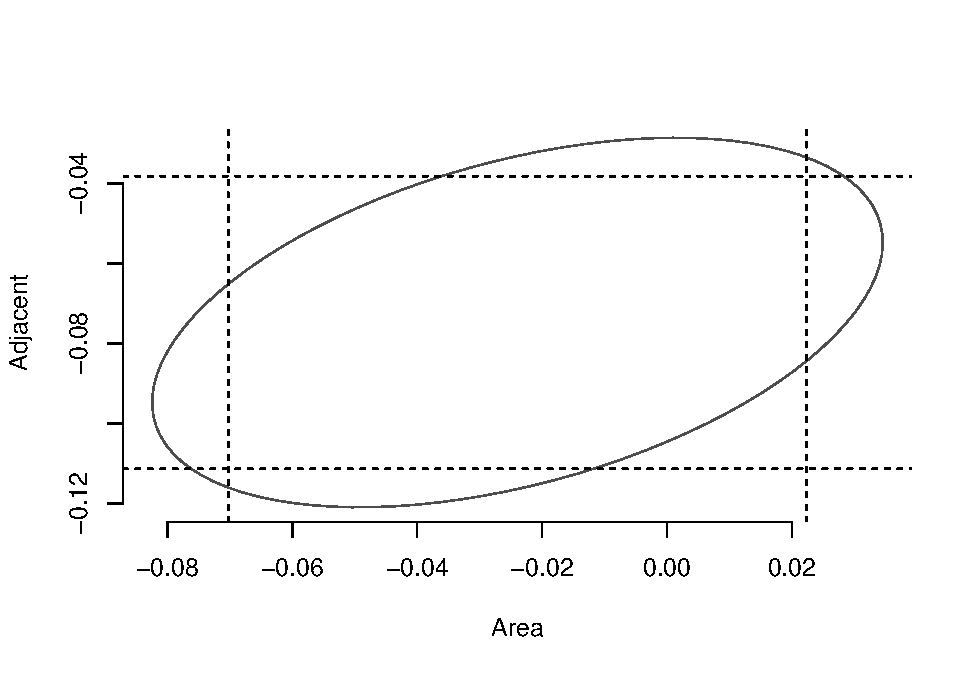
\includegraphics[width=0.9\linewidth]{Lab_9_10_files/figure-latex/unnamed-chunk-19-1} 

}

\caption{Regiune de incredere pentru Area si Adjacent}\label{fig:unnamed-chunk-19}
\end{figure}

Cum punctul \((0,0)\) nu aparține regiunii elipsoidale atunci putem
respinge ipoteza nulă \(H_0:\beta_{Area}=\beta_{Adjacent}=0\).


\end{document}
